%!TEX program = xelatex
% 完整编译: xelatex -> biber/bibtex -> xelatex -> xelatex
\documentclass[lang=cn,11pt,a4paper]{elegantpaper}

\title{有限元第三次编程作业}
\author{W Huang}
\date{\zhtoday}


% 本文档命令
\usepackage{array}
\usepackage{float}
\usepackage{multirow}
\usepackage{amsmath}
\usepackage{amssymb}
\newcommand{\ccr}[1]{\makecell{{\color{#1}\rule{1cm}{1cm}}}}

\begin{document}

\maketitle

\section{编程第一题}

\subsection{求解设置}

求解PDE
\begin{equation}
    \left\{
        \begin{array}{l}
            -\Delta u = f,\quad \text{in}\;\Omega=[0,1]^2,\\
            u = 0,\quad \text{on}\;\partial \Omega.
        \end{array}
    \right.
\end{equation}
取精确解
\begin{equation}
    u(x,y) = \sin(\pi x) \sin(\pi y),
\end{equation}
并导出右端项,进行测试。网格如图1所示。

\begin{figure}[H]
    \centering
    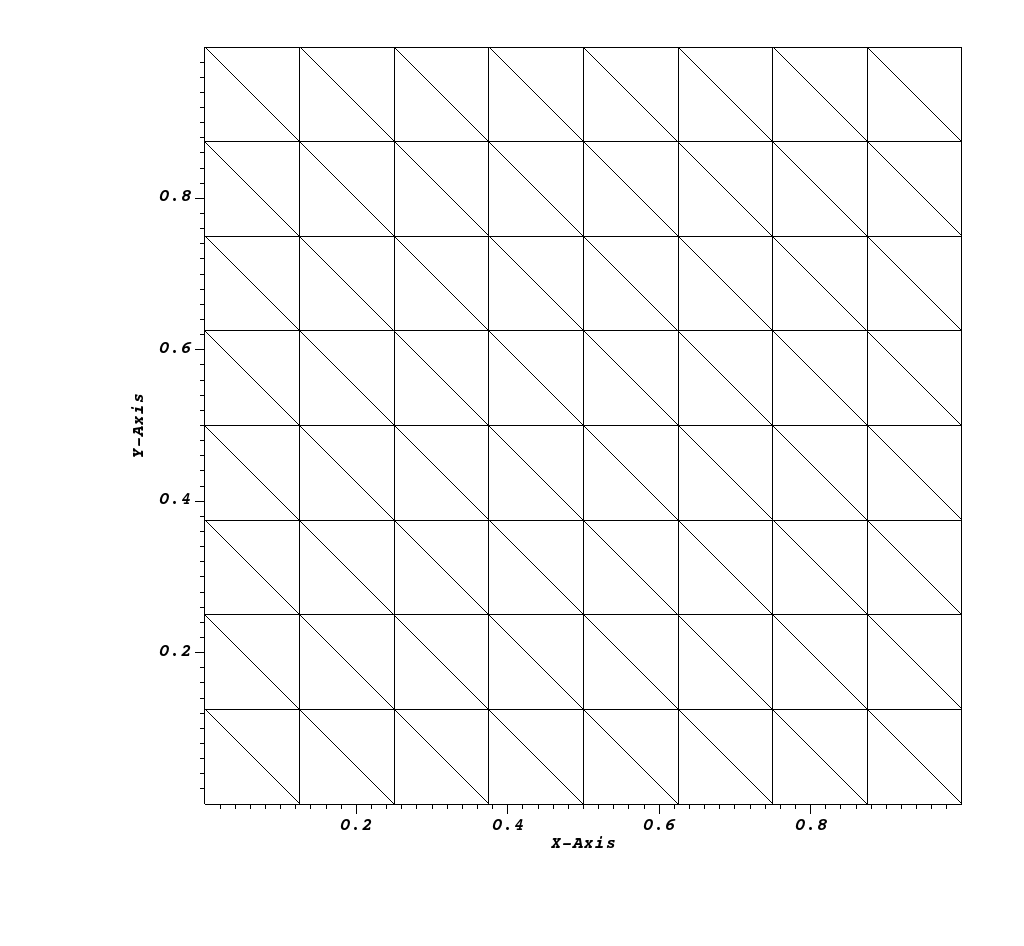
\includegraphics[width=0.5\textwidth]{png/mesh-2D.png}
    \caption{\small $h=\frac{1}{8}$ 时的计算网格}
\end{figure}

考虑 Hiercharchical Basis (以下简称HB) 预优算子:
\begin{equation}
    B=D+IA_H^{-1}I^t.
\end{equation}
其中 $I$ 是线性元空间下粗网格到细网格的自然延拓(即线性插值),而 $A_H^{-1}$ 涉及到
方程组的求解。我们选择使用\textbf{朴素 CG 方法}求解粗网格上的方程 $A_Hu_H=f_H$。

\subsection{编译说明}

请安装 deal.ii 及其依赖库,见 https://www.dealii.org/developer/readme.html;安装完毕后,在本文档目录下打开终端,依次运行:
\begin{lstlisting}
cd src-2D
mkdir build
cd build
cmake ..
make release
make
\end{lstlisting}
等待编译完成后,用以下命令执行测试:
\begin{lstlisting}
./elliptic 10 2
\end{lstlisting}
上述测试采用 1.1 节所述的网格,规模为 $N=2^{10}$,使用两层网格;
如果需要改变网格规模,将 \verb|10| 换成别的正整数;
如需使用多层网格,将 \verb|2| 换成别的正整数;
特别地,当最后一个参数缺省时,默认使用单层网格,即朴素 CG 方法。

\subsection{测试结果}

用朴素 CG 方法与 HB 预优 CG 方法对比,
Tolerance 设置为 $\varepsilon=10^{-12}||f||_2$ (其中 $f$ 是方程的右端项) 结果见图2,图3和表1。

可以看到,朴素 CG 方法的 CG 迭代次数指数级增长;HB 预优 CG 方法的 CG 迭代次数不升反降。
将预处理耗时与求解耗时相加,可以看出在 $h=1/1024$ 时,HB 预优 CG 方法具有明显加速。

首先我们需要说明,Tolerance 设置为 $\varepsilon=10^{-12}||f||_2$ 远远超过了实际需要,
其实想要达到上表的误差,Tolerance 设置为 $\varepsilon=10^{-4}||f||_2$ 足矣,求解几乎是瞬间完成。
我们取如此夸张的 Tolerance 是为了对比出加速效果。

但是,我们只取了两层网格,因此加速效果不明显。甚至当 $h$ 继续变小时,HB 预优 CG 方法
的速度比朴素 CG 方法还要慢。这是因为 HB 预优方法虽然最外层的 CG 迭代次数得到了控制,
但它需要在粗网格中进行大量的 CG 迭代,代价太大。
要在实际中应用,还是需要多层网格。

\vspace{-1em}

\begin{figure}[H]
    \centering
    \begin{minipage}[t]{0.4\textwidth}
        \centering
        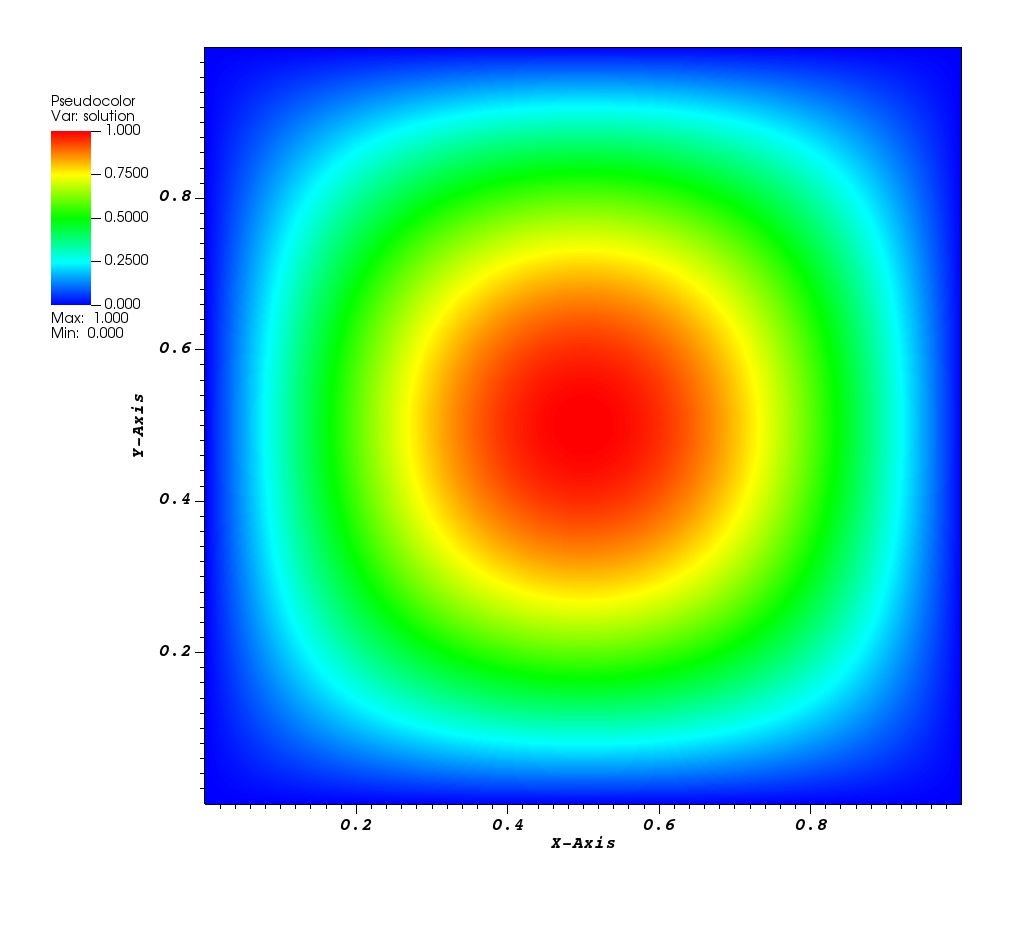
\includegraphics[width=\linewidth]{png/solution-2D.png}
        \caption{\small $h=\frac{1}{256}$时的数值解}
    \end{minipage}
    \hfill
    \begin{minipage}[t]{0.4\textwidth}
        \centering
        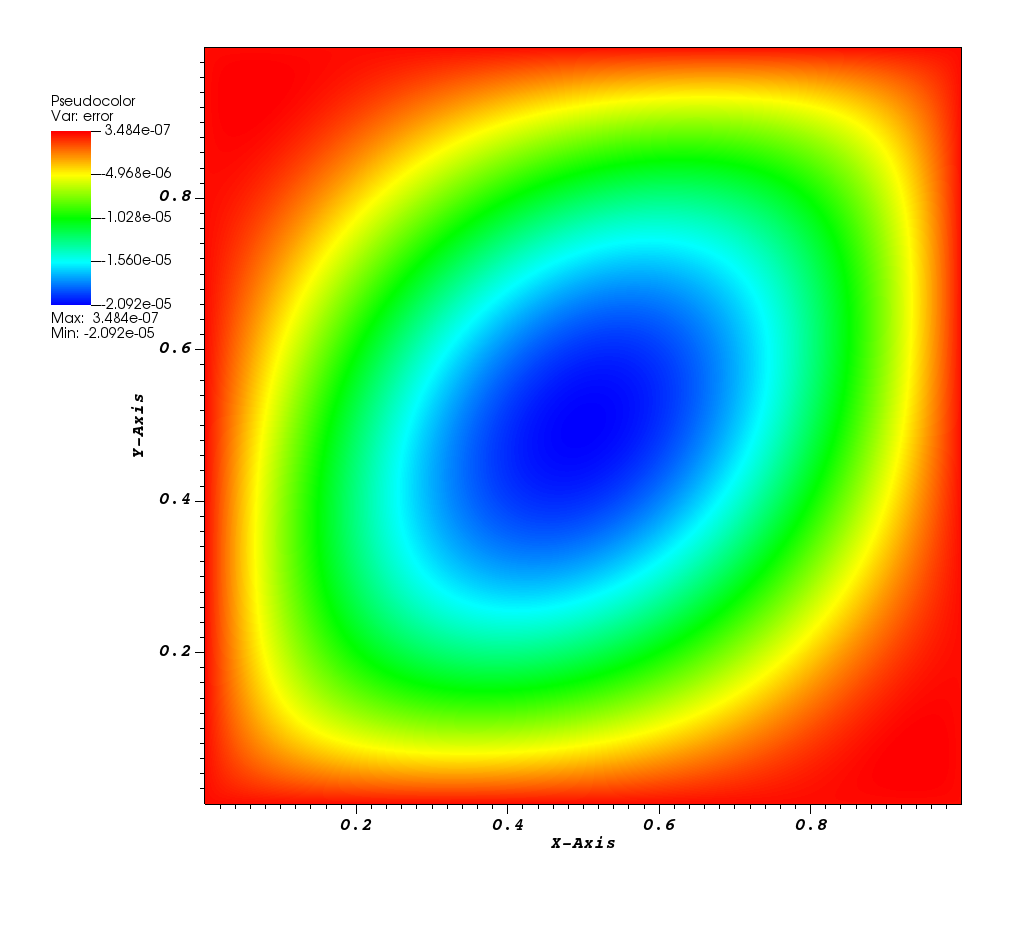
\includegraphics[width=\linewidth]{png/error-2D.png}
        \caption{\small $h=\frac{1}{256}$时数值解与真解的误差}
    \end{minipage}
\end{figure}

% Please add the following required packages to your document preamble:
% \usepackage{multirow}
\begin{table}[H]
    \centering
    \begin{tabular}{c|cccccc}
    \hline
                                                                                               & $h$               & $\frac{1}{256}$ & 收敛阶  & $\frac{1}{512}$ & 收敛阶  & $\frac{1}{1024}$ \\ \hline
    \multirow{5}{*}{朴素 CG 方法}                                                                  & $||u^h-u||_{L^2}$ & 2.46e-05        & 2.00 & 6.16e-06        & 2.00 & 1.54e-06         \\
                                                                                               & $||u^h-u||_{H^1}$ & 1.36e-02        & 1.00 & 6.82e-03        & 1.00 & 3.41e-03         \\
                                                                                               & 预处理耗时 (s)         & 0.23            &      & 0.92            &      & 3.9              \\
                                                                                               & 求解耗时 (s)          & 0.031           &      & 0.26            &      & 8.9              \\
                                                                                               & CG 迭代次数           & 439             &      & 852             &      & 1651             \\ \hline
    \multirow{5}{*}{\begin{tabular}[c]{@{}c@{}}HB 预优 CG 方法\\ (两层网格)\end{tabular}} & $||u^h-u||_{L^2}$ & 2.46e-05        & 2.00 & 6.16e-06        & 2.00 & 1.54e-06         \\
                                                                                               & $||u^h-u||_{H^1}$ & 1.36e-02        & 1.00 & 6.82e-03        & 1.00 & 3.41e-03         \\
                                                                                               & 预处理耗时 (s)         & 0.27            &      & 1.1             &      & 4.8              \\
                                                                                               & 求解耗时 (s)          & 0.10           &      & 0.84            &      & 3.6              \\
                                                                                               & CG 迭代次数           & 52              &      & 94              &      & 62               \\ \hline
    \multirow{5}{*}{\begin{tabular}[c]{@{}c@{}}HB 预优 CG 方法\\ (三层网格)\end{tabular}} & $||u^h-u||_{L^2}$ & 2.46e-05        & 2.00 & 6.16e-06        & 2.00 & 1.54e-06         \\
                                                                                               & $||u^h-u||_{H^1}$ & 1.36e-02        & 1.00 & 6.82e-03        & 1.00 & 3.41e-03         \\
                                                                                               & 预处理耗时 (s)         & 0.29            &      & 1.2             &      & 4.9              \\
                                                                                               & 求解耗时 (s)          & 0.15           &      & 0.68            &      & 3.0              \\
                                                                                               & CG 迭代次数           & 52              &      & 50              &      & 49               \\ \hline
    \end{tabular}
    \caption{\small $h=\frac{1}{256},\frac{1}{512},\frac{1}{1024}$ 的求解结果}
\end{table}

\section{编程第二题}

\subsection{求解设置}

求解PDE
\begin{equation}
    \left\{
        \begin{array}{l}
            -\Delta u = f,\quad \text{in}\;\Omega=[0,1]^3,\\
            u = 0,\quad \text{on}\;\partial \Omega.
        \end{array}
    \right.
\end{equation}
取精确解
\begin{equation}
    u(x,y,z) = 10 \sin(\pi x) \sin(\pi y) \sin(\pi z),
\end{equation}
并导出右端项,进行测试。三维空间中的四面体网格过于复杂,
粗细网格之间的索引极其困难,因此为了简化,我们选择了使用
六面体网格,如图4所示。

\vspace{-1em}
\begin{figure}[H]
    \centering
    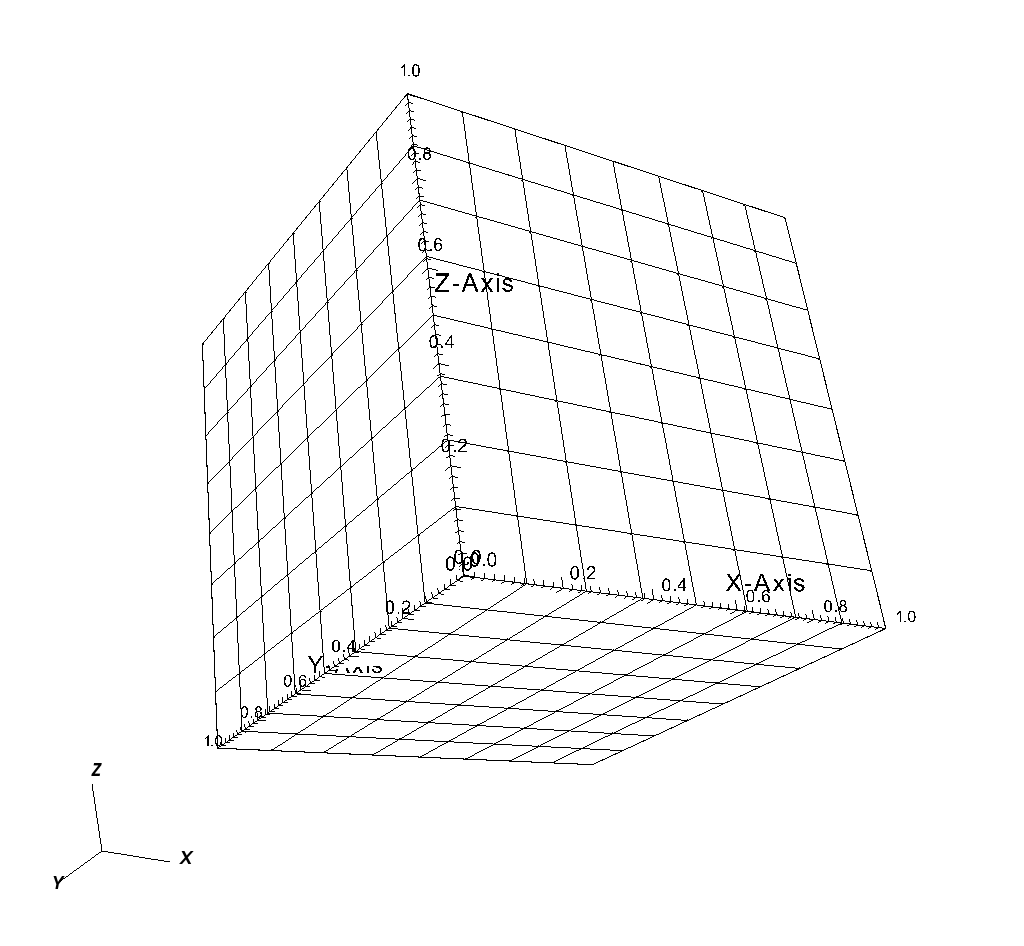
\includegraphics[width=0.4\textwidth]{png/mesh-3D.png}
    \caption{\small $h=\frac{1}{8}$ 时的计算网格}
\end{figure}

六面体网格对应的有限元空间是$Q_1$元,在$Q_1$元中,
对于一个参考单元$[0,1]^3$,其节点基函数为:
\begin{align*}
    \phi_{(0,0,0)}(x,y,z)&=(1-x)(1-y)(1-z),\\
    \phi_{(0,0,1)}(x,y,z)&=(1-x)(1-y)z,\\
    \phi_{(0,1,0)}(x,y,z)&=(1-x)y(1-z),\\
    \phi_{(0,1,1)}(x,y,z)&=(1-x)yz,\\
    \phi_{(1,0,0)}(x,y,z)&=x(1-y)(1-z),\\
    \phi_{(1,0,1)}(x,y,z)&=x(1-y)z,\\
    \phi_{(1,1,0)}(x,y,z)&=xy(1-z),\\
    \phi_{(1,1,1)}(x,y,z)&=xyz.
\end{align*}
在六面体网格和$Q_1$元下,粗细网格之间的索引非常容易,且线形插值的表示也非常简单。

考虑 Hiercharchical Basis (以下简称HB) 预优算子:
\begin{equation}
    B=D+IA_H^{-1}I^t.
\end{equation}
其中 $I$ 是线性元空间下粗网格到细网格的自然延拓(即线性插值),而 $A_H^{-1}$ 涉及到
方程组的求解。我们选择使用\textbf{朴素 CG 方法}求解粗网格上的方程 $A_Hu_H=f_H$。

编译、运行方法与二维程序完全相同,这里不做重复说明。

\subsection{测试结果}

用朴素 CG 方法与 HB 预优 CG 方法对比,
Tolerance 设置为 $\varepsilon=10^{-6}||f||_2$ (其中 $f$ 是方程的右端项) 结果见表2。

结论是两层网格的 HB 预优 CG 方法一致收敛,但与朴素 CG 方法相比,毫无加速效果。
另外,我们观察到朴素 CG 方法的迭代次数不随网格加细而增加,甚至稳定在 1 次,
这是一个有趣的现象。

\begin{table}[H]
    \centering
    \begin{tabular}{c|cccccc}
    \hline
                                                                                               & $h$               & $\frac{1}{32}$ & 收敛阶  & $\frac{1}{64}$ & 收敛阶  & $\frac{1}{128}$ \\ \hline
    \multirow{5}{*}{朴素 CG 方法}                                                                  & $||u^h-u||_{L^2}$ & 2.84e-03        & 2.00 & 7.10e-04        & 2.00 & 1.77e-04         \\
                                                                                               & $||u^h-u||_{H^1}$ & 5.45e-01        & 1.00 & 2.73e-01        & 1.01 & 1.36e-01         \\
                                                                                               & 预处理耗时 (s)         & 0.13            &      & 1.2            &      & 10              \\
                                                                                               & 求解耗时 (s)          & 0.00061           &      & 0.0044            &      & 0.035              \\
                                                                                               & CG 迭代次数           & 1             &      & 1             &      & 1             \\ \hline
    \multirow{5}{*}{\begin{tabular}[c]{@{}c@{}}HB 预优 CG 方法\\ (两层网格)\end{tabular}} & $||u^h-u||_{L^2}$ & 2.84e-03        & 2.00 & 7.10e-04        & 2.00 & 1.77e-04         \\
                                                                                               & $||u^h-u||_{H^1}$ & 5.45e-01        & 1.00 & 2.73e-01        & 1.01 & 1.36e-01         \\
                                                                                               & 预处理耗时 (s)         & 0.16            &      & 1.3             &      & 11              \\
                                                                                               & 求解耗时 (s)          & 0.0028           &      & 0.026            &      & 0.31              \\
                                                                                               & CG 迭代次数           & 4              &      & 4              &      & 4               \\ \hline
    \end{tabular}
    \caption{\small $h=\frac{1}{32},\frac{1}{64},\frac{1}{128}$ 的求解结果}
\end{table}

\appendix
%\appendixpage
\addappheadtotoc

\end{document}
